%%%%%%%%%%%%%%%%%%%%%%%%%%%%%%%%%%%%%%%%%%%%%%%%%%%%%%%%%%%%%%%%%%%%%%%%%%%%%%%%
%2345678901234567890123456789012345678901234567890123456789012345678901234567890
%        1         2         3         4         5         6         7         8

%\documentclass[letterpaper, 10 pt, conference]{ieeeconf} % Comment this line out
                                                          % if you need a4paper
\documentclass[a4paper, 10pt, conference]{ieeeconf}       % Use this line for a4
                                                          % paper

%\IEEEoverridecommandlockouts                              % This command is only
                                                          % needed if you want to
                                                          % use the \thanks command
\overrideIEEEmargins
\pagenumbering{arabic}
% See the \addtolength command later in the file to balance the column lengths
% on the last page of the document


% The following packages can be found on http:\\www.ctan.org
\usepackage{graphics} % for pdf, bitmapped graphics files
\usepackage{epsfig} % for postscript graphics files
\usepackage{mathptmx} % assumes new font selection scheme installed
\usepackage{times} % assumes new font selection scheme installed
\usepackage{amsmath} % assumes amsmath package installed
\usepackage{amssymb}  % assumes amsmath package installed
\usepackage{color}

\usepackage{comment}
%\usepackage{subfigure}
\usepackage{array}
\usepackage{float}
%\usepackage{caption}
\usepackage{algorithm}
\usepackage{algorithmic}
\usepackage{url}

\title{\LARGE \bf
TITLE
}

%\author{ \parbox{3 in}{\centering Huibert Kwakernaak*
%         \thanks{*Use the $\backslash$thanks command to put information here}\\
%         Faculty of Electrical Engineering, Mathematics and Computer Science\\
%         University of Twente\\
%         7500 AE Enschede, The Netherlands\\
%         {\tt\small h.kwakernaak@autsubmit.com}}
%         \hspace*{ 0.5 in}
%         \parbox{3 in}{ \centering Pradeep Misra**
%         \thanks{**The footnote marks may be inserted manually}\\
%        Department of Electrical Engineering \\
%         Wright State University\\
%         Dayton, OH 45435, USA\\
%         {\tt\small pmisra@cs.wright.edu}}
%}

%\author{ \parbox{3 in}{\centering Jeremie Deray
%		 \thanks{Universit\� de Bourgogne,
%        720 Avenue de l'Europe, 71200 Le Creusot, France
%        {\tt\small deray.jeremie@gmail.com}} } }
        
\author{Jeremie Deray {\tt\small deray.jeremie@iri.upc.edu}\\ Institut de Robotica i Informatica Industrial, CSIC-UPC.\\
Parc Tecnologic de Barcelona. C/ Llorens i Artigas 4-6. 08028 Barcelona, Spain\\ PAL Robotics, C/ Pujades 77-79, 08030 Barcelona, Spain}

\begin{comment}
\thanks{This work was not supported by any organization}% <-this % stops a space
\thanks{H. Kwakernaak is with Faculty of Electrical Engineering, Mathematics and Computer Science,
        University of Twente, 7500 AE Enschede, The Netherlands
        {\tt\small h.kwakernaak@autsubmit.com}}%
\thanks{P. Misra is with the Department of Electrical Engineering, Wright State University,
        Dayton, OH 45435, USA
        {\tt\small pmisra@cs.wright.edu}}%
}
\end{comment}

\begin{document}

\maketitle
\thispagestyle{empty}
\pagestyle{empty}

%%%%%%%%%%%%%%%%%%%%%%%%%%%%%%%%%%%%%%%%%%%%%%%%%%%%%%%%%%%%%%%%%%%%%%%%%%%%%%%%
\begin{abstract}

Robot localization during navigation is one of the fundamental problems of robot navigation. Topological localization characterizes the map nodes either in terms of global or local features extracted from sensor inputs. Following the local features approach, more precisely using the \textit{bag-of-word} scheme and its extension called \textit{Vocabulary-Tree} we focus in this paper on the geometrical check of the recognition pipeline. The use of a dynamic programing algorithm together with the way we define the problem allow for a fast assertion of basic geometrical characteristics while comparing local features of 2D range data. Moreover this geometrical test filters out some of the most critical erroneous feature matching that could occur. This last property allows then to solve an outlier free linar system for estimating the relative position of the robot.
RESULTS?

\end{abstract}

%%%%%%%%%%%%%%%%%%%%%%%%%%%%%%%%%%%%%%%%%%%%%%%%%%%%%%%%%%%%%%%%%%%%%%%%%%%%%%%%
\section{Introduction}
\label{chap:intro}

This is an introduction

\cite{Kosecka}


%%%%%%%%%%%%%%%%%%%%%%%%%%%%%%%%%%%%%%%%%%%%%%%%%%%%%%%%%%%%%%%%%%%%%%%%%%%%%%%%
\section{Chapter 1}
\label{sec:chap1}

\subsection{Subchapter1}
\label{sec:chap1sec1}

\subsection{Subchapter1}
\label{sec:chap1sec1}

\begin{equation}
	\sum_1^I \| T_{c1}^k \Delta T_i - \Delta T_i T_{ci}^k \|
\end{equation}

\begin{equation}
\Delta R = 
	\begin{bmatrix}
	-0.9998 & -0.0207 & -0.0026 \\
	-0.0209 &  0.9862 &  0.1642 \\
	-0.0008 &  0.1642 & -0.9864
	\end{bmatrix}
	\label{eq:matrix}
\end{equation}


%%%%%%%%%%%%%%%%%%%%%%%%%%%%%%%%%%%%%%%%%%%%%%%%%%%%%%%%%%%%%%%%%%%%%%%%%%%%%%%%
\section{Appearance-Based Place Recognition}
\label{sec:chap2}

The \textit{BoW} frameworks consists of two disctinct parts, firstly a set of cluster centers from the feature space so that $W=\{w_0, w_1,..., w_k\}$, also called visual words. It is constructed through a hierarchical \textit{K-means} in the same manner as \cite{Nister06} over a set of $20.000$ scans sampled from different datasets, with on average $17.5$ features per scan. The tree architecture has for parameters $K=?$ and $depth=?$ for a total of $?$ words.

The second part is a database and consists of a collection of documents so that $D=\{d_0, d_1,...\}$ and holds the known nodes of the map. Every node is a collection of descriptors extracted from the sensor reading, quantized into words using the above tree and become a document.

Within the database is kept a record of each word occurence in every documents so that as for text retrieval a \textit{Term Frequency} weight and an \textit{Inverse Document Frequency} weight can be associated to the word (\textit{tf-idf}).

At last, a document is characterized by a vector containing the \textit{tf-idf} weights and refered to as its signature. A documents comparison is performed by computing the $cos-similarity$ of their respective signatures.

Given a new sensor reading, its feature descriptors are extracted, converted into words and used to query the database. Its associated signature is computed and then compared to those of every documents in the database; the $N$ most similar documents are returned by the \textit{BoW} scheme.

%%%%%%%%%%%%%%%%%%%%%%%%%%%%%%%%%%%%%%%%%%%%%%%%%%%%%%%%%%%%%%%%%%%%%%%%%%%%%%%%
\section{Weak Geometrical Check}
\label{sec:chap3}

In this section we discuss the proposed geometrical check. First, we define 2D range data characteristics that similar scans must meet. Secondly, we define the problem as a Hidden Markov Model. Then the computation of the weak geometrical check and its implications.

\subsection{Observations}
\label{sec:obs}

Considering local features extracted from a 2D scan (quantized into words), in a clock-wise order as a 1D signal gives minimal geometric information. The order in which words appear must remain the same for a given scene observed from different viewpoints although it is subject to transfomation. This transformation is directly linked to the viewpoint transformation and occurs in the following manners:
\begin{itemize}
\item while observing a scene, a forward displacement of the sensor alongside its observation axis, words will tend to shift toward both extremum of the laser scan. Inversly, a backward displacement induces a shifting towards the center of the scan.
\item in case of a rotation in the plane, words are shifted in the laser scan entries - to the left for a clock-wise rotation, to the right for a counter-clockwise rotation. Whereas words can disappear from the readings and new ones appear due to large rotation, the remaining common observed words are solely shifted. Aside displacements produce the same observations.
\item any combination of the above displacements results in a combination of their respective transformations, ordering of word observation is then invariant to rotation and translation.
\item only cases of occlusion, changes in the environment and moving objects will lead to a change in the ordering.
\end{itemize}

\begin{figure}[ht]
\centering
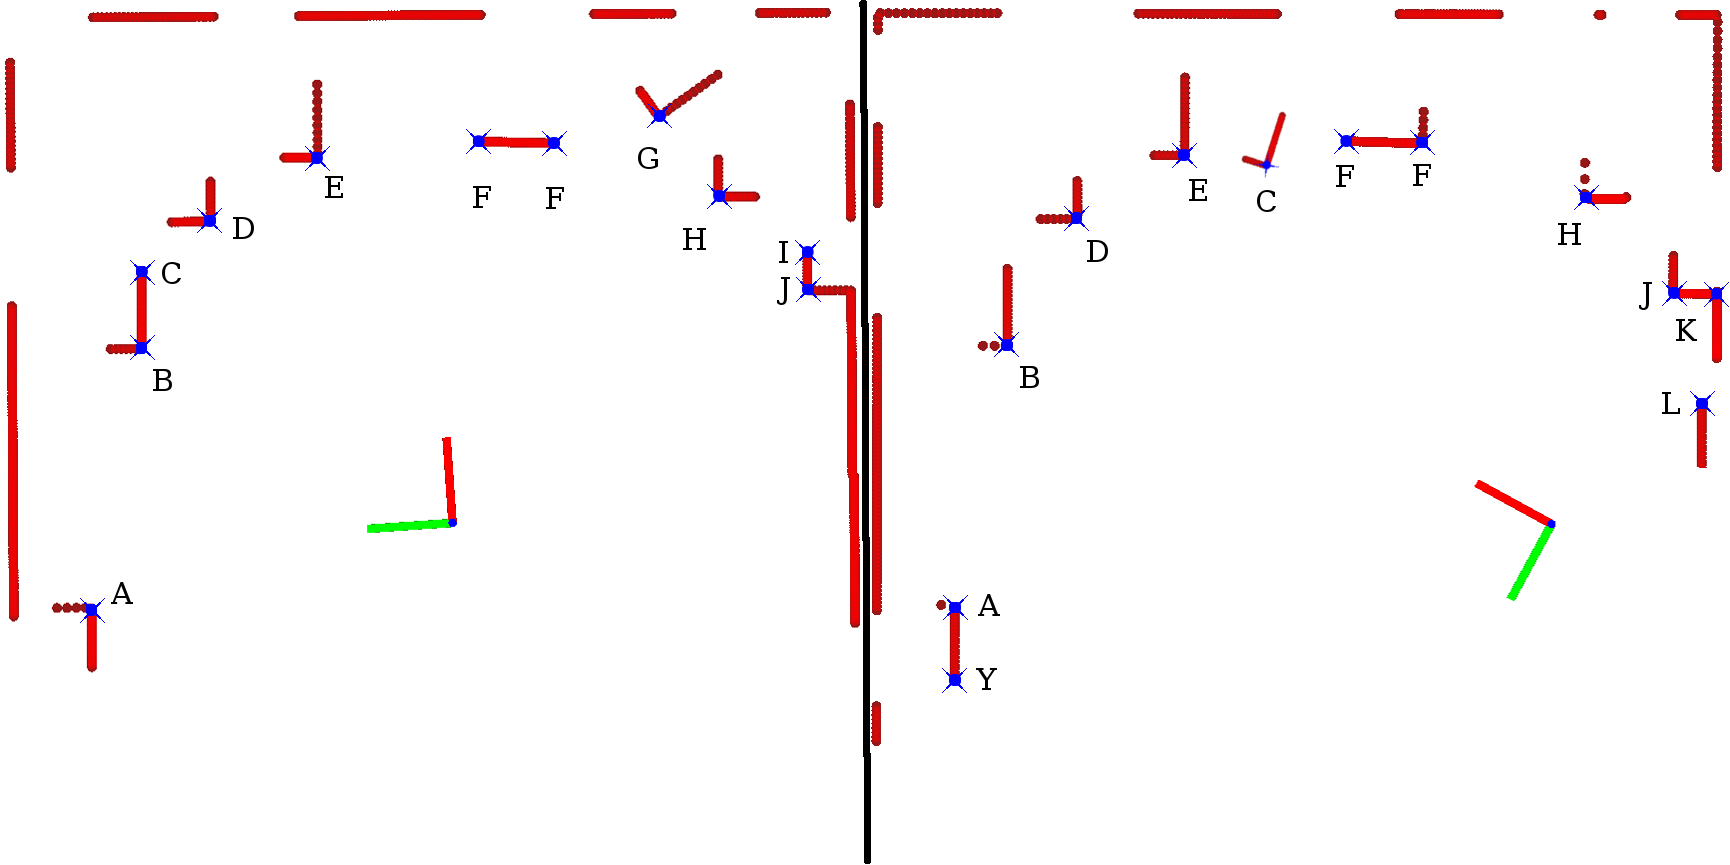
\includegraphics[width=1\linewidth]{image/merge.png}
\put(-200.0,0.0){\color[rgb]{0,0,0}{\makebox(1,1)[lb]{\smash{$x_i$}}}}
\put(-50.0,0.0){\color[rgb]{0,0,0}{\makebox(1,1)[lb]{\smash{$x_j$}}}}
\caption{Environment observed from two different viewpoints}
\label{fig:scans}
\end{figure}

\subsection{Matching and Ordering as a Hidden Markov Model}
\label{sec:hmm}

As mentioned in *ref.vocatree*, word matchings are directly given by the Vocabulary-Tree scheme. Together with their ordering they allow to define the problem as a graph - similar to a Hidden Markov Model (HMM) - from which a path that fully crosses it is maximized.

Considering the aser scan currently evaluated $x_i$ and its extracted words $W_N^{x_i}$ as a set of states $S_N$ and the candidate match $x_j$ with its words $W_M^{x_j}$ as a set of observations $O_M$ we can define our model such that:

\begin{itemize}
\item The states starting propabilities are all equal $\delta_{s_n} = 1/N$
\item The transition from a state to another can not go backward with respect to the clockwise ordering of the states. Transition probabilities are then defined such that ${\phi_{s_n,s_n}\to0.5}$, ${\phi_{s_n,s_{n+x}}\to1}$ whereas ${\phi_{s_{n-x},s_n}\to0}$
\item The output probability is defined such that a known mismatch has a very low probability whereas matches found by the Vocabulary-Tree have a very high probability. Emission probability will be defined for a match as ${\theta_{s_n,o_m}\to1}$ while for a mismatch ${\theta_{s_n,o_m}\to0}$
\end{itemize}

Figure\ref{fig:HMM} (top) shows the clockwise ordering of words extracted from both $x_i$ \& $x_j$ scans of Fig.\ref{fig:scans} with the matching produced by the Vocabulary-Tree.
Figure.\ref{fig:HMM} (middle) gives a simplified representation of the HMM produced by the current scan matching evaluation where $S_N$ are extracted $x_i$, $O_M$ extracted from $x_j$, black downward pointing arrows representing feasible transition, red upward pointing arrows representing non-feasible transitions. Each cell is then filled by the product
\begin{equation}
\label{eq:cellprod}
\phi_{s_n-x,s_n}*\theta_{s_n,o_m}
\end{equation}

Where $s_n$ is the currently evaluated state, $s_{n-x}$ is the previous optimal state and $o_m$ the output probability. Colums are filled recursively based on previous iteration.

Once the HMM is defined, the goal is then to find a sequence of state that maximise the probability of a path across it.

\subsection{The Viterbi algorithm}
\label{sec:viterbi}

In order to find the best path at a reasonable cost in terms of computation, we propose the use of a modified Viterbi algorithm \cite{Viterbi}. This dynamic programing algorithm searches recursively for the most likely sequence of states given a sequence of events by computing for each observation the partial probability with respect to the previous state that optimally induced the current state. It is commonly used in speech recognition, speech synthesis or decoding \cite{Rabiner} \cite{Shinghal}.

Crossing edges (Fig.\ref{fig:HMM}-top) highlight mismatching, either due to similar features that are quantized to the same word (e.g. words $C$ and $F$) or a moving object. Whereas \cite{TipaldiGFLIP} do not discard such mismatch while constructing their offset histogram, they must be discarded in order to compute a consistent relative transform. Thanks to the constraint of forward state transition, the Viterbi algorithm naturally discards such crossing. However it could discard one or the other of two crossing edges. In Fig.\ref{fig:HMM}-top it could either be preferable to keep the edge of the $C$ word and discard both $D$ and $E$ or the other way around. In order to emphasize strong matches we weigth Eq.\ref{eq:cellprod} by the word \textit{Inverse Document Frequency} \textit{(IDF)}. 
\begin{equation}
\label{eq:cellprodidf}
\phi_{s_n-x,s_n}*\theta_{s_n,o_m}.IDF(s_n)
\end{equation}

With $IDF(w_n)$ a function that returns the \textit{IDF} score of the word $w_n$ associated to state $s_n$.
Doing so, words that appear less frequently will be kept instead of more frequent ones. This relies on the assumption that words less frequently observed are related to more discriminative local features.

\begin{figure}[H]
\centering{
\resizebox{1\linewidth}{!}{\input{inkscape/drawing_0.pdf_tex}}
%\captionsetup{belowskip=-2cm}
%\hspace{2cm}
\caption{Top: Clockwise ordered words of two scans and their matches. Middle: The resulting Hidden Markov Model. Each cell represent the product ${\phi_{s_n-x,s_n}*\theta_{s_n,o_m}.IDF(s_n)}$ e.g cells \textit{Y-A} \& \textit{A-A}. Green squared cells represent the best path across the complete graph. Bottom: The final sequence of states given the observations $O_n$}
\label{fig:HMM}
}
\end{figure}

\subsection{Scoring}
\label{sec:viterbiscore}

Once the best path obtained, the candidate scoring is done on two criterions:
\begin{itemize}
\item the number of (correct) matches that have not been discarded by the Viterbi algorithm
\item the number of consecutive words that have a correct match
\end{itemize}

The latest point is analogue to the concept of phrases in \cite{TipaldiGFLIP} where a phrase $p^k$ represent a sequence of $k$ consecutive words. Considering such sequences and weighting them accordingly to their length add an extra layer of constraint to the geometrical check.

** can't give more details until a proper scoring is found.

\subsection{Experiments}
\label{sec:exp}

** To be defined

Same as \cite{TipaldiGFLIP} ? 

%%%%%%%%%%%%%%%%%%%%%%%%%%%%%%%%%%%%%%%%%%%%%%%%%%%%%%%%%%%%%%%%%%%%%%%%%%%%%%%%
\section{Conclusion}

conclusion ...


%%%%%%%%%%%%%%%%%%%%%%%%%%%%%%%%%%%%%%%%%%%%%%%%%%%%%%%%%%%%%%%%%%%%%%%%%%%%%%%%

% ***** bibliography *******
% **************************
\bibliographystyle{ieeetr}
\bibliography{bibliography.bib}

\end{document}